\documentclass{article}

% Recommended, but optional, packages for figures and better typesetting:
\usepackage{microtype}
\usepackage{graphicx}
\usepackage{subfigure}
\usepackage{booktabs} % for professional tables

% hyperref makes hyperlinks in the resulting PDF.
% If your build breaks (sometimes temporarily if a hyperlink spans a page)
% please comment out the following usepackage line and replace
% \usepackage{icml2018} with \usepackage[nohyperref]{icml2018} above.
\usepackage{hyperref}

% Attempt to make hyperref and algorithmic work together better:
\newcommand{\theHalgorithm}{\arabic{algorithm}}

% Use the following line for the initial blind version submitted for review:
%\usepackage{icml2018}

% If accepted, instead use the following line for the camera-ready submission:
\usepackage[accepted]{icml2018}

% The \icmltitle you define below is probably too long as a header.
% Therefore, a short form for the running title is supplied here:
\icmltitlerunning{Skin Cancer Detection using SLICE-3D Data (ISIC 2024)}

\begin{document}

\twocolumn[
\icmltitle{Skin Cancer Detection using SLICE-3D Data (ISIC 2024)}

% It is OKAY to include author information, even for blind
% submissions: the style file will automatically remove it for you
% unless you've provided the [accepted] option to the icml2018
% package.

% List of affiliations: The first argument should be a (short)
% identifier you will use later to specify author affiliations
% Academic affiliations should list Department, University, City, Region, Country
% Industry affiliations should list Company, City, Region, Country

% You can specify symbols, otherwise they are numbered in order.
% Ideally, you should not use this facility. Affiliations will be numbered
% in order of appearance and this is the preferred way.
\icmlsetsymbol{equal}{*}

\begin{icmlauthorlist}
\icmlauthor{Giovanni Budi}{da}
\icmlauthor{Andrew Chisolm}{mo}
\icmlauthor{Noah Parker}{mo}
\end{icmlauthorlist}

\icmlaffiliation{mo}{Molinaroli College of Engineering and Computing, University of Sourth Carolina, Columbia, South Carolina}
\icmlaffiliation{da}{Darla Moore School of Business, University of Sourth Carolina, Columbia, South Carolina}

\icmlcorrespondingauthor{Giovanni Budi}{gbudi@email.sc.edu}
\icmlcorrespondingauthor{Andrew Chisolm}{chisolmi@email.sc.edu}
\icmlcorrespondingauthor{Noah Parker}{nhparker@email.sc.edu}

% You may provide any keywords that you
% find helpful for describing your paper; these are used to populate
% the "keywords" metadata in the PDF but will not be shown in the document
\icmlkeywords{Machine Learning, ICML}

\vskip 0.3in
]

% this must go after the closing bracket ] following \twocolumn[ ...

% This command actually creates the footnote in the first column
% listing the affiliations and the copyright notice.
% The command takes one argument, which is text to display at the start of the footnote.
% The \icmlEqualContribution command is standard text for equal contribution.
% Remove it (just {}) if you do not need this facility.

\printAffiliationsAndNotice{}  % leave blank if no need to mention equal contribution
%\printAffiliationsAndNotice{\icmlEqualContribution} % otherwise use the standard text.

\begin{abstract}
    This paper evaluates a skin cancer detection system aimed at overcoming accessibility challenges in underserved
    regions. Utilizing the ISIC SLICE-3D dataset, which consists of smartphone-quality images, the system employs
    EfficientNet architectures to classify skin lesions as malignant or benign. We compare models trained on high-quality
    2019 ISIC data, smartphone-quality 2024 ISIC data, and a fine-tuned transfer learning model to assess their
    performance. Our results demonstrate the promise of transfer learning in enhancing diagnostic accuracy and
    specificity, while addressing challenges related to class imbalance and data variability.
\end{abstract}

\section{Introduction}
\label{introduction}

Skin cancer remains a global health challenge, with early detection playing a vital role in improving survival rates. Despite advancements in dermoscopic imaging that have enhanced diagnostic accuracy, the reliance on specialized equipment limits accessibility, particularly in underserved regions. The lack of affordable and practical diagnostic tools prevents early intervention, exacerbating the burden of skin cancer in resource constrained settings. Addressing the gap requires innovative solutions that can adapt to the realities of limited medical infrastructure.

Our project aims to tackle this issue by developing an accessible and robust skin cancer detection system that leverages smartphone-quality images. The SLICE-3D dataset was created for the 2024 International Skin Imaging Collaboration (ISIC) competition and features images of such quality. We employ EfficientNet architectures to classify images of skin lesions from this dataset as malignant or benign. By comparing models trained on high-quality 2019 ISIC data with those trained on lower-quality 2024 ISIC data, we explore the potential of transfer learning to bridge the gap in diagnostic accuracy between datasets of differing quality. This approach seeks to make advanced diagnostic capabilities more widely available, even in areas lacking specialized imaging equipment.

To achieve this, we followed a systematic methodology. First, we replicated the ISIC 2019 winner's methodology using the 2019 dataset transformed into binary classifications. Next, we tested the model’s performance on the 2024 dataset to evaluate the impact of image quality. Finally, we fine-tuned the pretrained 2019 model on the 2024 dataset to enhance its performance on lower-quality images. This step-by-step approach allowed us to assess the impact of image quality and transfer learning while addressing challenges such as class imbalance and data variability, ultimately contributing to the development of a more inclusive and effective diagnostic system.

\section{Related Work}

There has been ample research in recent years on machine learning approaches to identifying different types of skin cancer. This paper primarily builds off of the work of Gessert et.\ al.\ in their submission that won the ISIC 2019 challenge \yrcite{gessert20}. ISIC holds a skin imaging challenge every year, with each challenge receiving entries from thousands of participants. Participants in these challenges employ a wide range of novel techniques to better classify skin lesions. EfficientNets~\cite{pmlr-v97-tan19a} have been proven to be an effective architecture in accurately classifying the images~\cite{venugopal2023deep,ali2022multiclass,sm2023classification}. Researchers have also had success using transfer learning based methods on some of the same datasets used in this study~\cite{moldovan2019,bassi2019}.

There have been several attempts at creating a smartphone application that uses AI algorithms to detect skin cancer based on an image taken from the smartphone, to varying degrees of success~\cite{wolf2013diagnostic,maier2015accuracy,udrea2020accuracy,chuchu1996smartphone}. Each of these papers cite room for improvement in either the sensitivity or specificity of their results.

\section{Data}

This paper utilizes two datasets, both used in ISIC challenges. The first is from ISIC’s 2019 challenge. The 2019 data is the collection of high quality, dermoscopic images from the 
BCN\_20000 Dataset, the HAM10000 Dataset, and the MSK Dataset~\cite{bcn20000,ham10000,msk}. These data were collected from the Hospital Clínic in Barcelona, the Department of 
Dermatology at the Medical University of Vienna, Austria, the skin cancer practice of Cliff Rosendahl in Queensland, Australia, and the Memorial 
Sloan-Kettering Cancer Center in New York. The 25,331 total images were captured using dermatoscopes at these labs and contain features not visible to the naked eye. They were labeled into nine different 
categories, some benign and some malignant. Metadata relating to the demographics of the patient were also included.

The second dataset utilized in this paper is the 3D SLICE dataset, used in ISIC’s 2024 challenge. Rather than being captured from a dermatoscope, these images were extracted from 3D total body photographs~\cite{slice3d}. The 400,000 images are cropped to a 15 mm x 15 mm scale, and they closely resemble the quality of a smartphone camera. The images were gathered from nine sites in Australia, Europe, and the United States.


\section{Experimentation}

\subsection{Experimental Setup}

To validate the methodology and ensure proper setup, we first replicated Gessert et.\ al.'s ISIC 2019 experiment,
using the skin lesion categories provided in the dataset. This process involved carefully aligning file locations,
model parameters, and software packages to the specifications detailed in the paper. Once replication was
completed, we adapted the dataset to our specific goal: binary classification of malignant vs. benign skin lesions.
This enabled a direct comparison of the 2019 and 2024 datasets under consistent conditions.

\subsection{Data Preperation}

The ISIC 2019 dataset initially contained nine different multi-class labels for various skin lesion types. To meet our binary
classification objective, we transformed the dataset by mapping each lesion category to either ``malignant'' or
``benign''. This transformation was guided by medical domain knowledge and consistent with classifications used
in prior research. After transformation, the dataset was restructured and split into trainin g and validation sets.

The ISIC 2024 dataset, in contrast, already provided binary classification labels, eliminating the need
for additional transformation. We directly utilized the dataset for training and evaluation, focusing on addressing
its challenges, such as lower image quality and significant class imbalance (1:20 malignant-to-benign ratio).

\subsection{Binary Classification Models}

We trained three distinct models for binary classification:

\subsubsection{ISIC 2019 Model}

\begin{itemize}

\item Trained exclusively on the 2019 dataset with the binary-transformed labels, leveraging its high-quality
images and balanced (1:2 malignant-to-benign) class ratio.
\item Based on the pretrained EfficientNet-B0 and fine-tuning on the 2019 dataset to adapt to its specific features.

\end{itemize}

\subsubsection{ISIC 2024 Model}

\begin{itemize}

\item Trained on the 2024 dataset with no label transformation, addressing its significant class imbalance
(1:20 ratio) and smartphone-quality images.
\item Follows the same pretrained EfficientNet-B0 backbone and fine-tuning on the
2024 dataset to handle the challenges of lower-quality images and class imbalance.

\end{itemize}

\subsubsection{Fine-Tuned 2019/2024 Model}

\begin{itemize}

\item This model is based on the best-performing 2019 model, which has been pretrained on the ISIC 2019
dataset and fine-tuned for optimal performance.
\item For the 2019/2024 Fine-Tuned Model, we froze certain layers of the 2019 model, including the
conv\_stem, block 0, and block 1 layers, while fine-tuning the higher layers on the ISIC 2024 dataset.
This allows the model to retain the general features learned from the 2019 dataset while adapting to the
more challenging 2024 dataset.

\end{itemize}

\subsection{Image Preprocessing for Training and Validation}

\subsubsection{Training}

During training, the following transformations are applied to augment the dataset and improve model
generalization:

\begin{itemize}

\item \textbf{Random Resized Crop:} Randomly resizes and crops the image to a specified size, improving the
model's robustness to different scales.
\item \textbf{Random Flip:} Random horizontal and vertical flips to increase the variety of image orientations.
Rotation: Random rotation (within a specified range) to improve the model's invariance to rotation.
\item \textbf{ColorJitter:} Random adjustments to the brightness, contrast, saturation, and hue of the image to
simulate different lighting conditions.
\item \textbf{Cutout:} Randomly masks out a portion of the image, forcing the model to focus on less prominent
features and improve generalization.
\item \textbf{Normalization:} Normalizes the pixel values according to the dataset's mean and standard deviation to
standardize the input for the model.
\item \textbf{ToTensor:} Converts the image to a PyTorch tensor, which is the format required for input into the
model.

\end{itemize}

\subsubsection{Validation}

During validation, the following transformations are applied to ensure consistent, deterministic behavior while
still allowing some degree of variability:

\begin{itemize}

\item \textbf{CenterCrop:} Crops the image to a fixed size from the center to ensure a consistent region of interest is
evaluated.
\item \textbf{Fixed Crops:} When necessary, crops the image at predefined, deterministic positions for validation.
\item \textbf{Flipping:} Horizontal flip may be applied for testing, but this is generally less aggressive than in
training.
\item \textbf{Normalization:} Normalizes the image using the same mean and standard deviation as used in training.
\item \textbf{ToTensor:} Converts the image to a tensor for use in evaluation.

\end{itemize}

\subsection{Training and Validation}

Each model was evaluated using a 5-fold cross-validation framework to ensure robustness and generalizability
across unseen data. Training parameters, data augmentation techniques, and class weights were carefully
optimized to mitigate the challenges posed by the datasets. The Cross-Entropy Loss with Class Weights was
used during training to address the class imbalance, particularly in the 2024 dataset, where the malignant -to-
benign ratio is 1:20.

Detailed metrics for all models and folds are summarized in Tables~\ref{2019table},~\ref{2024table}, and~\ref{20192024table}, and discussed in subsequent
sections. The results highlight the performance trade-offs between datasets, models, and configurations,
providing a clear pathway for further optimization in clinical contexts.

The following training parameters were employed to ensure the model trained efficiently while mitigating
overfitting and achieving optimal performance:

\begin{itemize}
    \item \textbf{Batch Size:} 20
    \item \textbf{Initial Learning Rate:} 0.000015
    \item \textbf{Learning Rate Adjustment:} After 25 epochs with no improvement, the learning rate was reduced by a
factor of 5.
    \item \textbf{Training Steps:} 60 epochs
    \item \textbf{Mean and Standard Deviation for Normalization:} Set to [0.0, 0.0, 0.0] and [1.0, 1.0, 1.0] respectively,
ensuring the input images were normalized accordingly
\end{itemize}

These parameters were essential to managing the training process, ensuring stability, and preventing overfitting,
especially with the imbalanced data.

\subsection{Evaluation Setup}

We employed a diverse set of metrics, including accuracy, sensitivity, specificity, AUC, and ROC curve
analysis, to comprehensively evaluate our models' performance in predicting these classifications.

\begin{itemize}
    \item \textbf{Accuracy:} The percentage of correct predictions over the total dataset.
    \item \textbf{Sensitivity:} The proportion of malignant cases correctly identified.
    \item \textbf{Specificity:} The proportion of benign cases correctly identified.
    \item \textbf{Area Under the Curve (AUC):} Measures the trade-off between sensitivity and specificity, evaluating
model discrimination.
    \item \textbf{ROC Curve Analysis:} Graphical representation of model performance across classification thresholds.
    \item \textbf{Class-Wise Precision and Recall:} Evaluates per-class performance, particularly important for
addressing class imbalance.
\end{itemize}

\begin{figure}[h]
    \label{eval_plot}
    \caption{Evaluation metrics for the three models.}
    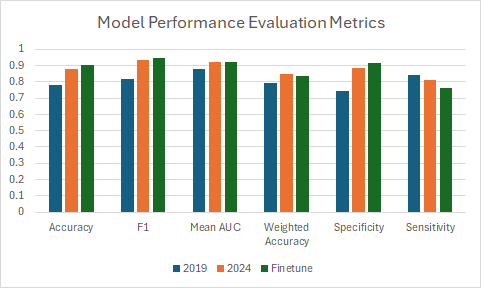
\includegraphics[width=8cm]{model-performance.png}
\end{figure}

\section{Positive Outcomes}

Our evaluation of the 2019, 2024, and fine-tuned 2019/2024 models demonstrates several key strengths in handling
varying image qualities and class imbalances:

\begin{enumerate}
    \item \textbf{Improved Performance with Fine-Tuning:} The fine-tuned 2019/2024 model outperformed both the
standalone 2019 and 2024 models, achieving a 2.3\% increase in accuracy and a 1.4\% increase in F1 score.
This highlights the value of fine-tuning and transfer learning in adapting the model to the 2024 dataset,
even with lower-quality images.
    \item \textbf{Enhanced Specificity:} The fine-tuned model exhibited a notable improvement in specificity, rising by 2.8\%
compared to the 2024 model. This suggests that the model is more effective at distinguishing between
benign and malignant cases, reducing the number of false positives.
    \item \textbf{Effective Transfer Learning:} The success of the fine-tuned model indicates that leveraging the 2019
model’s architecture and weights provided valuable knowledge transfer, enabling the model to better
handle the challenges posed by the 2024 dataset with smartphone-quality images.
\end{enumerate}

\section{Limitations}

Despite these positive outcomes, certain limitations need attention:

\begin{enumerate}
    \item \textbf{Lower Sensitivity:} Both the 2024 model and the fine -tuned 2019/2024 model exhibited a drop in
sensitivity, particularly the fine-tuned model, which showed a decrease of 5.4\%. This could be attributed to
the extreme class imbalance in the 2024 dataset (1:20 ratio of malignant to benign cases), which likely
hindered the model’s ability to detect malignant cases as effectively.
    \item \textbf{Class Imbalance Impact:} The sensitivity issue underscores the challenge posed by class imbalance, which
impacted the model's ability to identify malignant cases, especially in the 2024 dataset. The relatively
balanced 1:2 ratio in the 2019 dataset did not face this issue to the same extent, contributing to better
sensitivity in that model.
\end{enumerate}

These results suggest that while transfer learning and fine-tuning have significantly improved specificity and overall
accuracy, further efforts are needed to address the sensitivity issue, likely through strategies for mitigating class
imbalance.

\section{Chameleon Cloud Feedback}

We started using Chameleon Cloud for this project as a way to avoid having to run the program on our own devices. There was a fairly steep learning curve to get started. In particular, we had difficulty in getting multiple users to access the same instance once we had a reservation set up. To work around this issue, we ended up fooling the computer into thinking we were all the same user by all using a single public and private key, which most certainly is not the intended approach. We also failed to properly back up our files before one instance ended. Once an instance ends, Chameleon Cloud provides no way to get the files back, so we ended up losing some progress. The sum of all these technical difficulties motivated us to switch to doing our computation on Kaggle instead.

With some more patience and foresight, we likely could have used Chameleon Cloud more effectively, but given our time constraints, we opted to stick with what we were familiar with, which was functional enough for the purposes of this project.

\begin{table*}[t]
    \caption{2019 Model Results}
    \label{2019table}
    \vskip 0.15in
    \begin{center}
    \begin{small}
    \begin{sc}
    \begin{tabular*}{\linewidth}{@{\extracolsep{\fill}} cccccccc}
    \toprule
    Fold & Epoch & Accuracy & F1 & Mean AUC & Weighted Accuracy & Specificy & Sensitivity \\
    \midrule
    0 & 60 & 0.7735 & 0.8114 & 0.8826 & 0.7934 & 0.7330 & 0.8538 \\
    1 & 60 & 0.7777 & 0.8138 & 0.8812 & 0.7971 & 0.7365 & 0.8576 \\
    2 & 60 & 0.7811 & 0.8241 & 0.8699 & 0.7857 & 0.7717 & 0.7998 \\
    3 & 60 & 0.7833 & 0.8212 & 0.8835 & 0.7993 & 0.7503 & 0.8483 \\
    4 & 60 & 0.7799 & 0.8164 & 0.8780 & 0.7967 & 0.7435 & 0.8500 \\
    \midrule
    &    & 0.7791 & 0.8174 & 0.8790 & 0.7944 & 0.7470 & 0.8419 \\
    \bottomrule
    \end{tabular*}
    \end{sc}
    \end{small}
    \end{center}
    \vskip -0.1in
\end{table*}

\begin{table*}[t]
    \caption{2024 Model Results}
    \label{2024table}
    \vskip 0.15in
    \begin{center}
    \begin{small}
    \begin{sc}
    \begin{tabular*}{\linewidth}{@{\extracolsep{\fill}} cccccccc}
    \toprule
    Fold & Epoch & Accuracy & F1 & Mean AUC & Weighted Accuracy & Specificy & Sensitivity \\
    \midrule
    0 & 30 & 0.8752 & 0.9308 & 0.9045 & 0.8249 & 0.8805 & 0.7692 \\
    1 & 20 & 0.8940 & 0.9420 & 0.9334 & 0.8637 & 0.8966 & 0.8308 \\
    2 & 30 & 0.9104 & 0.9507 & 0.9411 & 0.8716 & 0.9153 & 0.8280 \\
    3 & 30 & 0.8715 & 0.9283 & 0.9055 & 0.8435 & 0.8745 & 0.8125 \\
    4 & 40 & 0.8624 & 0.9229 & 0.9316 & 0.8476 & 0.8640 & 0.8312 \\
    \midrule
      &    & 0.7791 & 0.8174 & 0.8790 & 0.7944 & 0.7470 & 0.8419 \\
    \bottomrule
    \end{tabular*}
    \end{sc}
    \end{small}
    \end{center}
    \vskip -0.1in
\end{table*}

\begin{table*}[t]
    \caption{2019/2024 Fine Tuned Model Results}
    \label{20192024table}
    \vskip 0.15in
    \begin{center}
    \begin{small}
    \begin{sc}
    \begin{tabular*}{\linewidth}{@{\extracolsep{\fill}} cccccccc}
    \toprule
    Fold & Epoch & Accuracy & F1 & Mean AUC & Weighted Accuracy & Specificy & Sensitivity \\
    \midrule
    0 & 40 & 0.8873 & 0.9379 & 0.9186 & 0.8312 & 0.8932 & 0.7692 \\
    1 & 60 & 0.9116 & 0.9523 & 0.9319 & 0.8212 & 0.9193 & 0.7231 \\
    2 & 50 & 0.9122 & 0.9518 & 0.9373 & 0.8625 & 0.9185 & 0.8065 \\
    3 & 30 & 0.9188 & 0.9560 & 0.9016 & 0.8446 & 0.9268 & 0.7625 \\
    4 & 60 & 0.9024 & 0.9468 & 0.9166 & 0.8253 & 0.9104 & 0.7403 \\
    \midrule
      &    & 0.9065 & 0.9490 & 0.9212 & 0.8370 & 0.9136 & 0.7603 \\
    \bottomrule
    \end{tabular*}
    \end{sc}
    \end{small}
    \end{center}
    \vskip -0.1in
\end{table*}

\section{Conclusions and Future Steps}

Although class weighting was implemented in the loss function to address the class imbalance, the extreme
imbalance in the 2024 dataset (1:20 ratio) may still have hindered the model’s ability to detect malignant cases
effectively. The class weights helped by giving more importance to the minority class, but the disparity between
malignant and benign cases might still pose challenges for detection. Further techniques, such as oversampling the
minority class, more aggressive class balancing, or modifications to the model architecture, could be explored to
enhance sensitivity for malignant cases.

Another potential contributing factor to the lower sensitivity is the nature of the 2024 dataset, which consists of
smartphone-quality images. These images may contain less detail or more noise compared to the high resolution
images from the 2019 dataset, which could further complicate the model’s ability to detect subtle features associated
with malignant lesions. While the fine-tuned model improved specificity and accuracy, enhancing sensitivity for
malignant cases remains a priority for future work.

Overall, the fine-tuned 2019/2024 model provided the best balance of performance, particularly in terms of
specificity. This outcome underscores the benefits of transfer learning, where leveraging the 2019 model’s learned
features helped improve performance on the lower-quality 2024 images. However, the drop in sensitivity signals a
potential area for further refinement. While class weighting in the loss function helped mitigate the impact of class
imbalance, the extreme imbalance in the 2024 dataset remains a challenge.

To address the lower sensitivity for malignant cases, future work will explore additional techniques such as more
aggressive class balancing, oversampling, or further fine-tuning the model to better capture subtle malignant
features. Additionally, further experiments could evaluate whether image quality improvement techniques, such as
data augmentation or super-resolution methods, could help the model better handle the lower-quality 2024 images
and enhance its sensitivity.

By continuing to refine the model’s ability to detect malignant cases, we hope to achieve better overall performance
and greater generalization across datasets with varying image quality.


\section{Acknowledgements}
This project could not have been completed without the continued support and guidance of Dr.\ Pooyan Jamshidi. We also want to acknowledge our classmates, who offered helpful feedback and suggestions throughout the semester.

% In the unusual situation where you want a paper to appear in the
% references without citing it in the main text, use \nocite
\nocite{gessert20}

\bibliography{skin_cancer_detection}
\bibliographystyle{icml2018}


\end{document}


% This document was modified from the file originally made available by
% Pat Langley and Andrea Danyluk for ICML-2K. This version was created
% by Iain Murray in 2018. It was modified from a version from Dan Roy in
% 2017, which was based on a version from Lise Getoor and Tobias
% Scheffer, which was slightly modified from the 2010 version by
% Thorsten Joachims & Johannes Fuernkranz, slightly modified from the
% 2009 version by Kiri Wagstaff and Sam Roweis's 2008 version, which is
% slightly modified from Prasad Tadepalli's 2007 version which is a
% lightly changed version of the previous year's version by Andrew
% Moore, which was in turn edited from those of Kristian Kersting and
% Codrina Lauth. Alex Smola contributed to the algorithmic style files.
